\chapter{Traffic Congestion}

\resp{Marco Tavis Foster}



\section{Introduction}
    In this project we explore the effects of traffic congestion in a complex system \cite{Arenas2001} \cite{Echenique2004}. We will work with a hierarchical network structure and explore how the dynamical system evolves as 'packets' move through it in discrete time steps. We impose that the probability of a packet moving from its current node to a target node is determined by a weight, which is affected by the number of packets already in the current node. The effect is that, as the number of packets in a node grows, the transmissibility decreases exponentially. In this way we witness the effect of traffic congestion on the dynamical processes in a complex network.

\section{Method}

    We begin by selecting the network structure itself, expressly one best suited to witness the movement of the packets and the effects of packet overload. To this end a hierarchical tree structure is chosen; this forces the packets to move through one path as there is only a single path between any pair of nodes. Furthermore, we expect that the root will likely be the first to be overloaded as any packet that needs to travel to the other half of the network must go through the root. Intuitively we can imagine this as the lines of communication between employees at a company, with packets representing information.
    There are two factors in a tree network structure we can vary:

\begin{itemize}
  \item z = branching factor (number of children each node has)
  \item m = number of levels 
\end{itemize}

For our results we will be working with z = 3 and m = 3 - G(z, m) = G(3, 3). A visual representation of this graph can be seen in Fig. 2.1.

\begin{figure}[h] 
  \centering
  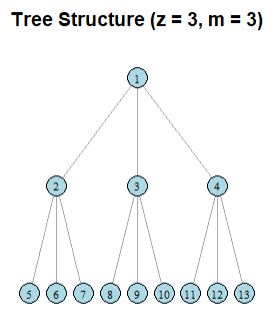
\includegraphics[width=0.6\textwidth]{images/Tree Structure.png} % Replace with your image filename
  \caption{This is the caption of the figure.}
  \label{fig:example}
  \end{figure}

    An important part of our process is the initialisation of packets. At each time step a packet is created at each node with probability p, and when a packet is generated we assign it a 'destination node' that is not the same as the origin node.
    At each time step it is also important to move the packets.  This is determined by the 'quality of communication, given by:
\begin{equation}
    q_{ij} =  \sqrt{k_{ij}k_{ji}}
\end{equation}
where $k_{ij}$, the capability for i to communicate with j, is given by:
\begin{equation}
    k_{ij} = \xi_{ij}f(n_a)
\end{equation}
where $\xi_{ij}$ is a uniformly distributed number between 0 and 1, and $f(n_a)$ is a function that we can select. In this project we elected to set it to:

$f(n_a) =$
\begin{cases}
    1 & \text{for } n = 0 \\
    n^{-\gamma} & \text{otherwise}
\end{cases}

with $\gamma \geq 0$.

    Moving the packet involves the following procedure. First we compute the shortest path (in this case the only path) between its current node and its destination, and we select the next node in the shortest path as the 'target node'. The packet - with probability $q_{ij}$ - moves to this target node. If the target node is the same as the destination mode the packet is 'delivered' and removed from the network. This procedure, along with the generation of new packets, is repeated for $n$ time steps.

\begin{figure}[H]
  \centering

  \begin{minipage}[t]{0.45\textwidth}
    \centering
    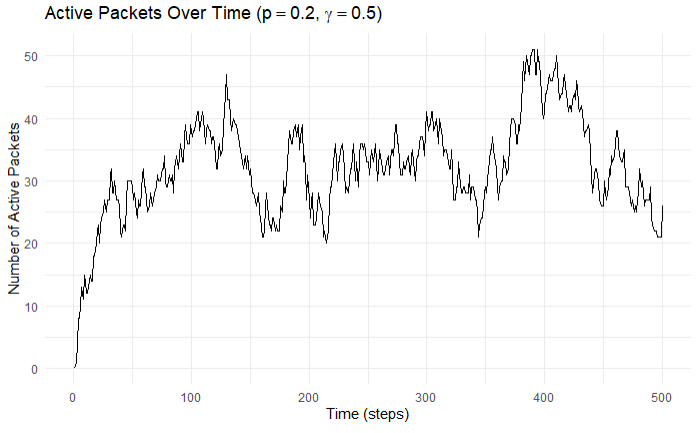
\includegraphics[width=\linewidth]{images/p02y05.png}
    \caption{Sytem evolution for p = 0.2 and $\gamma$ = 0.5}
    \label{fig:image1}
  \end{minipage}
  \hfill
  \begin{minipage}[t]{0.45\textwidth}
    \centering
    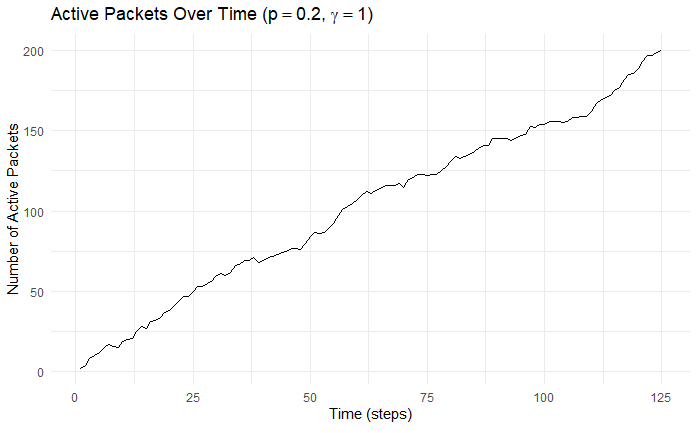
\includegraphics[width=\linewidth]{images/p02y1.png}
    \caption{Sytem evolution for p = 0.2 and $\gamma$ = 1}
    \label{fig:image2}
  \end{minipage}
  \hfill
  \begin{minipage}[t]{0.45\textwidth}
    \centering
    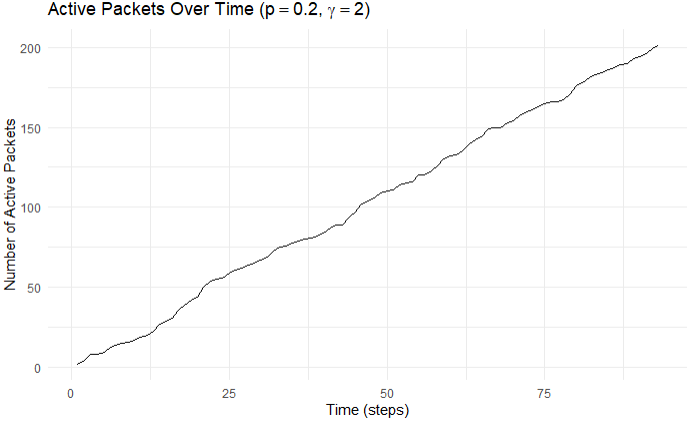
\includegraphics[width=\linewidth]{images/p02y2.png}
    \caption{System evolution for p = 0.2 and $\gamma$ = 2}
    \label{fig:image3}
  \end{minipage}
\caption{State evolution when the packet generation probability is kept constant and $\gamma$ is varied. Here we explore three regimes; Fig 2.2) $\gamma \leq 1$, Fig 2.3) $\gamma = 1$, Fig 2.4) $\gamma \geq 1$}
\end{figure}

For our simulations we explore three regimes:
\begin{enumerate}
    \item $\gamma < 1$: The number of transmitted packets grow as $n_a$ does. Thus the number of delivered packets increases as N grows until an equilibrium between delivered and generated packets is reached.
    \item $\gamma = 1$:  The number of delivered packets is constant irrespective of the number of packets already in the system.
    \item $\gamma > 1$: The number of delivered packets decreases as $n_a$ does. We therefore expect a dependence on the generation probability in regards to the evolution of the system. If $p$ is small enough the system can handle the number of packets travelling through it and so a steady state is reached. However, if $p$ is large enough then the system will become overloaded - the number of packets in the system will become so large that everything is blocked and eventually no packets can be delivered.
\end{enumerate}

We define $p_c$, the criticality threshold for the initialising probability. Above this value we expect the bottleneck root node to be overloaded and travelling through it to become impossible. This is given by:

$p_c = \frac{\sqrt{z}}{\frac{z(z^{m-1} - 1)^2}{z^{m-1}} + 1}$

For our network (z = m = 3) $p_c = 0.2065749$.

Finally, I was curious if the breakdown of communication through the root node would cause a cascade failure through the network - where the system is able to bare the 'load' right up until one node no longer functions properly, at which point more nodes fail in a cascade. In our case we do not see this as one node failing does not put additional strain on its neighbouring nodes (for example, by sharing out packets to neighbouring nodes once the node fails). We could explore the effects of an overloaded node on the ability of its neighbouring nodes to communicate with it by modifying the ratio between $k_{ij}$ and $k_{ji}$, which would change whether communication depends more on the number of packets at the current node or the number of packets at the target node.

\newpage